%\VignetteIndexEntry{Using Yadayada}
%\VignetteEngine{R.rsp::tex}
\documentclass[nojss]{jss}
%% -- LaTeX packages and custom commands ---------------------------------------
\usepackage{thumbpdf,lmodern}
\usepackage{framed}
\usepackage{amsmath}
\newcommand{\class}[1]{`\code{#1}'}
\newcommand{\fct}[1]{\code{#1()}}
\usepackage{multirow}
\usepackage{graphicx}
\usepackage{bm}
\usepackage{amssymb}
\usepackage{amsthm}
\newtheorem{definition}{Definition}
\usepackage{hyperref}
\newtheorem{theorem}{Theorem}[section]

\usepackage{xpatch}
\makeatletter
\AtBeginDocument{\xpatchcmd{\@thm}{\thm@headpunct{.}}{\thm@headpunct{}}{}{}}
\makeatother

\author{Marco Battaglini\\Cornell University, EIEF and NBER
	\And Valerio Leone Sciabolazza\\University of Naples Parthenope \AND Eleonora Patacchini\\ Cornell University, EIEF \And Sida Peng\\Microsoft Research}
\Plainauthor{Marco Battaglini, Valerio Leone Sciabolazza, Eleonora Patacchini, Sida Peng}

\title{\pkg{econet}: An \proglang{R} package for parameter-dependent network centrality measures}
\Plaintitle{\pkg{econet}: An R package for parameter-dependent network centrality measures}
\Shorttitle{\pkg{econet}: An \proglang{R} package for parameter-dependent network centrality measures}

\Abstract{
	The \proglang{R} package \pkg{econet} provides methods for estimating parameter-dependent network centrality measures with linear-in-means models. Both nonlinear least squares and maximum likelihood estimators are implemented. The methods allow for both link and node heterogeneity in network effects, endogenous network formation and the presence of unconnected nodes. The routines also compare the explanatory power of parameter-dependent network centrality measures with those of standard measures of network centrality. Benefits and features of the \pkg{econet} package are illustrated using data from \cite{Battaglini+Patacchini:2018}, which examine the determinants of US campaign contributions when legislators care about the behavior of other legislators to whom they are socially connected.
}

\Keywords{network econometrics, heterogeneous peer effects, endogenous network formation, least-square estimators, maximum likelihood estimators, R}
\Plainkeywords{network econometrics, heterogeneous peer effects, endogenous network formation, least-square estimators, maximum likelihood estimators, R}

\Address{
	Marco Battaglini\\
	Department of Economics\\
	Cornell University\\
	Ithaca, NY 14850, USA\\
	\emph{and} EIEF \emph{and also} NBER\\
	E-mail: \email{battaglini@cornell.edu}\newline
	\\
	Valerio Leone Sciabolazza\\
	Department of Business and Economics\\ 
	University of Naples Parthenope\\
	Naples, 80132, Italy\\
	E-mail: \email{valerio.leonesciabolazza@parthenope.it}\newline
	\\
	Eleonora Patacchini\\
	Department of Economics\\
	Cornell University\\
	Ithaca, NY 14850, USA\\
	\emph{and} EIEF\\
	E-mail: \email{ep454@cornell.edu}\newline
	\\
	Sida Peng\\
	Office of Chief Economist\\
	Microsoft Research\\
	Redmond, WA 14865, USA\\
	E-mail: \email{sidpeng@microsoft.com}
}

\shortcites{spdep}
\shortcites{statnet}
\begin{document}
	
	\section{Introduction} \label{sec:intro}
	
	Since its inception, network analysis has mostly focused on the discovery of topological properties of network structures. This has changed dramatically over the past ten years. An emerging literature in economics has shown that network centrality measures, which were traditionally viewed as descriptive, have an interpretation within equilibrium models of behavior. The pioneer paper is \cite{Ballester+Armengol+Zenou:2006}. This paper considers a model in which an agent's effort is triggered by the effort of his/her socially connected peers. It shows that the equilibrium outcome is a linear function of the agent's position in the network as measured by an indicator within the family of Katz-Bonacich centralities. Katz-Bonacich centralities 
	\citep{Katz:1953,Bonacich:1972,Bonacich:1987} are network centrality measures that count all nodes that can be reached through a direct or indirect path, penalizing in different ways the contributions of distant nodes in determining a given node's centrality.  The discount factor is captured by a parameter, thus making the measures of centrality parameter-dependent. The sociological literature has been treating this parameter as a nuisance parameter, and arbitrarily setting it to any value smaller than one. However, the contribution of \cite{Ballester+Armengol+Zenou:2006} is to show that this parameter captures the strength of peer effects or social interactions that stem from the aggregation of dyadic peer influences. More specifically, the empirical counterpart of the \cite{Ballester+Armengol+Zenou:2006} equilibrium condition is a linear model of social interactions, where the individual outcome is a linear function of the outcomes of the connected agents. The parameter capturing this influence is then used to measure the individual's importance in the network. Since then, a burgeoning empirical literature has used the linear-in-means model to prove that peer effects and the individual position in the social network play an important role in explaining many social and economic outcomes, including consumer behavior, voting patterns, job search, information diffusion, innovation adoption, international trade and risk sharing \citep[see e.g.,][for recent reviews]{Jackson+Rogers+Zenou:2017,Zenou:2016}
	
	Very recently \cite{Battaglini+Patacchini:2018} present a new theory of competitive vote-buying to study how interest groups allocate campaign contributions when legislators care about the behavior of other legislators to whom they are socially connected. The model provides an alternative microfoundation for network measures within the family of Katz-Bonacich centralities. This theory predicts that, in equilibrium, campaign contributions are proportional to a parameter-dependent measure of network centrality, similar to the one proposed by \cite{Ballester+Armengol+Zenou:2006}. While \cite{Ballester+Armengol+Zenou:2006} is a purely theoretical paper, \cite{Battaglini+Patacchini:2018} test the theory with data from five recent U.S. Congresses. In doing so, it confronts a variety of empirical challenges. For example, the theories described above show the importance of combining the information on network centrality with additional information on characteristics of the agents, since these characteristics can magnify or reduce the role played by a central agent. Moreover, the theories provide a framework to study the role of network endogeneity. In fact, when agents are strategic in choosing their peers, and omitted variables (such as social skills) drive both agent's behavior and social connectedness, the estimation of the peer effects parameter might be flawed \citep{Manski:1993}.
	
	The routines contains in the package \pkg{econet} for \proglang{R} \citep{R} allow for implementation of a number of variations of the linear-in-means model to obtain alternative centrality measures within the family of Katz-Bonacich centrality. Both nonlinear least squares (NLLS) and maximum likelihood (ML) estimators are provided. Several methods for dealing with the identification of network effects are implemented. Moreover, the \pkg{econet} package allows for comparison of the explanatory power of parameter-dependent network centrality measures with those of standard measures of network centrality \citep{Wasserman+Faust:1994}. As a result, \pkg{econet} expands the large set of tools available to \proglang{R} users interested in network analysis. Specifically, it has at least four merits. First, it complements the \proglang{R} packages implementing traditional centrality measures for binary networks, \pkg{igraph} \citep{igraph} and \pkg{sna} \citep{sna}, and weighted networks, \pkg{tnet} \citep{tnet}, by introducing new eigensolutions-based techniques to rank agents' centrality. Second, whereas previous packages, such as \pkg{btergm} \citep{btergm}, \pkg{hergm} \citep{hergm}, the \pkg{statnet} suite \citep{statnet}, and \pkg{xergm} \citep{xergm}, created environments for modeling the statistical processes underlying network formation, \pkg{econet} provides the first framework to investigate the socio-economic processes operating on networks (i.e., peer effects). Third, it completes the collection of functions for modeling spatial dependence in cross-sectional data provided by \pkg{spdep} \citep{spdep} and \pkg{splm} \citep{splm}, by allowing the users to: i) consider the presence of unconnected nodes, and ii) address network endogeneity. Finally, it equips the \proglang{R} archive with routines still unavailable in other commonly used software for the investigation of relational data, such as \proglang{MATLAB} \citep{MATLAB}, \proglang{Pajek} \citep{Batagelj:2003}, \proglang{Python} \citep{Python} and \proglang{Stata} \citep{Stata}. The example we use to showcase the functionality of our \proglang{R} package is taken from \cite{Battaglini+Patacchini:2018} and \cite{Battaglini+Sciabolazza+Patacchini:2018}. The \proglang{R} package \pkg{econet} is available from the Comprehensive R Archive Network at \url{https://CRAN.R-project.org/package=econet} 
	
	The rest of the paper is organized as follows. Section \ref{sec:models} briefly reviews the key elements for the estimation of parameter-dependent centralities, and presents a general taxonomy of the different approaches used to model the socio-economic processes operating on the network. Section 3 lays out various models and methods to deal with network endogeneity. Section 4 demonstrates the use of the main functions of the package \pkg{econet} to determine agent's centrality with examples. Section 5 concludes.
	
	%% -- Manuscript 
	
	\section{Network models of peer effects} \label{sec:models}
	Let $N=\left\{ 1,\ldots ,n\right\} $ be a finite set of agents in a network $g\equiv g_{N}.$ We keep track of connections in the network $g$ through its adjacency matrix $\boldsymbol{G}$ $=[g_{ij}]$\textbf{,} where $g_{ij}=1$ if $ i$ is connected to $j$ ($j\neq i$) and $g_{ij}=0$ otherwise. We set $g_{ii}=0$. For each network $g$ with adjacency matrix $\boldsymbol{G}=[g_{ij}]$, the $k$th power of $\boldsymbol{G}$ given by $\boldsymbol{G}^{k}= \boldsymbol{G}\overset{(k\text{times})}{\boldsymbol{...}}\boldsymbol{G}$ keeps track of direct and indirect connections in $g$. More precisely, the $(i,j)$th cell of $\boldsymbol{G}^{k}$ gives the number of paths of length $k$ in $g$ between $i$ and $j$. In particular, $\boldsymbol{G}^{0}=\boldsymbol{I}$.
	
	\begin{definition}[Katz, 1953; Bonacich, 1987] \label{Def1}
		Given a vector $\boldsymbol{u}\in \mathbb{R}_{+}^{n}$, and $\phi\geq 0$ a small enough scalar, the vector of Katz-Bonacich centralities of parameter $\phi$ in network $g$ is defined as: 
		\begin{equation}
		\boldsymbol{b}\left( g,\phi \right) =\left( \boldsymbol{I}-\phi \boldsymbol{G}\right) ^{-1}\boldsymbol{u=}\sum\limits_{p=0}^{\infty}\phi ^{p}%
		\boldsymbol{G}^{p}\boldsymbol{u}.  
		\label{KB}
		\end{equation}
	\end{definition}
	
	The first order necessary and sufficient condition for optimality in the behavioral model developed by \cite{Battaglini+Patacchini:2018}, BP henceforth, can be written as:
	\begin{equation}
	\mathbf{y}_{\mathbf{r}}=\alpha \cdot \left( \boldsymbol{I}-\phi \boldsymbol{G%
	}\right) ^{-1}+X_{r}^\top\mathbf{\beta }+\mathbf{\epsilon }_{r},
	\label{s_r_2}
	\end{equation}
	where $\mathbf{y}_{\mathbf{r}}$ is the vector of outcomes for the $n$ players in network $r\mathbf{,}$ $X_{r}$ is a matrix collecting the characteristics of the agents and $\mathbf{\epsilon }_{r}$ is a random error term. The coefficients $\alpha $, $\phi $ and $\mathbf{\beta }$ are the parameters to estimate. Model~\ref{s_r_2} can be written as
	\begin{equation}
	\mathbf{y}_{r}=\alpha \cdot \boldsymbol{b}_{1}\left( g,\phi \right)
	+X_{r}^\top\mathbf{\beta }+\mathbf{\epsilon }_{r},
	\end{equation}%
	where $\boldsymbol{b}_{1}\left(g,\phi \right) =\boldsymbol{b}\left(g,\phi
	\right) $ from equation~\ref{KB} when $\boldsymbol{u}=1$.\newline
	For a sample with $\bar{r}$ networks, one can stack up the data by defining $y=(\mathbf{y}_{1}^\top,\cdots$,$\mathbf{y}_{\bar{r}}^\top)^\top$, $\mathbf{\epsilon }=(\boldsymbol{\epsilon }_{1}^\top,\cdots ,\boldsymbol{\epsilon }_{_{\bar{r}}}^\top)^\top$, $\mathbf{b}(\phi)=\left(\boldsymbol{b}\left(g,\phi \right)^\top,...,\boldsymbol{b}\left(g,\phi\right)^\top\right) ^\top$, $G=\mathrm{diag}\{\boldsymbol{G}_{r}\}_{r=1}^{_{\bar{r}}}$, and $X=(\boldsymbol{X}_{1}^\top,...,\boldsymbol{X}_{\overline{r}}^\top)$. For the entire sample, the model is: 
	\begin{equation}
	y=\alpha \cdot \mathbf{b(}\phi \mathbf{)}+X\mathbf{\beta}+\mathbf{\epsilon }  \label{NLLS}
	\end{equation}
	We extend model~\ref{NLLS} by accounting for heterogeneity in network spillovers. Specifically, model~\ref{NLLS} becomes:
	\begin{equation}
	y=\alpha \lbrack I-G(\phi I+\gamma \Lambda )]^{-1}1+X\mathbf{\beta }+\mathbf{\epsilon }  
	\label{BP_2}
	\end{equation}
	where $\Lambda =I\otimes z$ is a matrix with the values in the vector $z$ on the diagonal, and all other values are 0. The vector $z$ represents a given characteristic of the agents. Consistently, the term $\gamma$ allows for the possibility that agents with different characteristics may be more or less susceptible to social spillovers.
	
	The first order necessary and sufficient condition for optimality in the behavioral model developed by \cite{Battaglini+Sciabolazza+Patacchini:2018}, BLP henceforth, is: 
	\begin{equation}
	\mathbf{y}_{r}=\left(I-\phi G\right) ^{-1}(\alpha
	+X_{r}^\top\mathbf{\beta )}+\mathbf{\epsilon }_{r}
	\label{BLP0}
	\end{equation}
	which can be rewritten as:
	\begin{equation}
	\mathbf{y}_{r}=\boldsymbol{b}_{2}\left( g,\phi \right)+\mathbf{\epsilon}_{r}  
	\label{BLP}
	\end{equation}
	where $\boldsymbol{b}_{2}\left( g,\phi \right) =\boldsymbol{b}\left( g,\phi
	\right) $ from (\ref{KB}) when $\boldsymbol{u}=(\alpha +\boldsymbol{X}_{r}^\top\mathbf{\beta)}$. Equation~\ref{BLP} shows that, in this case as well, the optimal behavior is proportional to a centrality measure within the Family~\ref{KB}.
	When we consider the case where the parameter $\phi$ associated with network externalities is not constant across agents, model~\ref{BLP} in matrix formulation becomes:
	\begin{equation}
	y=(I-\theta \Lambda G)^{-1}(\alpha +X\mathbf{\beta })+\mathbf{\epsilon}
	\label{BLP_3a}
	\end{equation}
	\begin{equation}
	y=(I-\eta G\Lambda)^{-1}(\alpha +X\mathbf{\beta })+\mathbf{\epsilon}
	\label{BLP_3b}
	\end{equation}
	In equations ~\ref{BLP_3a} and \ref{BLP_3b}, $\Lambda $\ is a diagonal matrix of ones. In equation~\ref{BLP_3a}, $\theta =\theta _{0}+\theta _{1}z$, where $\theta _{0}$\ is a rescaling factor, and $\theta _{1}$ quantifies the interaction between the adjacency matrix $G$ and the vector $z$. Consequently, $\theta _{1}$ measures the extent to which the peers of an agent with a given characteristic are susceptible to her/his influence. Similarly, in equation~\ref{BLP_3b}, $\eta =\eta _{0}+\eta _{1}z$, where $\eta _{0}$ is a rescaling factor, and $\eta _{1}$ measures the extent to which an agent with a given characteristic $z$ is more susceptible to the influence of her/his peers.
	
	In addition, BLP also consider the possibility of heterogeneous links (rather than nodes). We consider the case in which agents belong to two different groups and interactions are different between and within groups. To allow for group effects, one can reorder the matrix $G$ so that the first $n_{1}$ columns refer to agents in the first group, and the other $n_{2}=n-n_{1}$ columns refer to agents in the second group. The matrix $G$ can now be divided into four submatrices. The submatrices in the main diagonal (of dimensions $n_{1}\cdot n_{1}$ and $n_{2}\cdot n_{2})$ collect the interactions within groups, whereas the remaining two submatrices (of dimensions $n_{1}\cdot n_{2}$ and $n_{2}\cdot n_{1})$ collect interactions
	between groups. $G$ can thus be decomposed in two $n\cdot n$ matrices $G_{wit}$ and $G_{btw}$, with $G=G_{wit}+G_{btw}$. $G_{wit}$\ is a matrix that has the same top left and bottom right components as $G$ and it is zero otherwise, and $G_{btw}$ is a matrix that has the same bottom left and top right components as $G$ and it is zero otherwise. As a result, model ~\ref{BLP} becomes
	\begin{equation}
	y=(I-\phi _{1}G_{wit}-\phi _{2}G_{btw})^{-1}(\alpha +X\mathbf{\beta })+ \mathbf{\epsilon }  \label{BLP_4}
	\end{equation}
	where $\phi _{1}$ captures within-group spillovers, and $\phi _{2}$ between-group spillovers.
	The taxonomy of models outlined above shows that centrality measures should be calculated according to the most appropriate behavioral model describing the agents' behaviors and the requested level of heterogeneity of agents and network links. In BP and BLP we bring these theories to the data and find support for their predictions in different contexts.
	
	\subsection{Estimation} \label{sec:estimation}
	
	Models~\ref{NLLS} and \ref{BLP} cannot be estimated by a simple OLS regression in which $\mathbf{y}$ represents the dependent variables and $\mathbf{b}(\phi)$ and $X$ are the independent variables because $\mathbf{b}(\phi)$ is a nonlinear function of a parameter to be estimated, $\phi $. We can, however, obtain estimates for $\alpha $, $\phi$ and $\mathbf{\beta}$ using NLLS or ML.
	
	The NLLS requests solving the nonlinear least-squares problem for equation~\ref{NLLS} and~\ref{BLP}. This task is performed by \pkg{econet} using the Levenberg-Marquardt algorithm implemented in the \proglang{R} package \pkg{minpack.lm} developed by \cite{minpack.lm}.
	
	The ML estimation requests ML functions that can be derived as follows, by assuming $\mathbf{\varepsilon}\sim N(0,\sigma ^{2}I).$ For equation~\ref{NLLS}, assume $\mathbf{\varepsilon }\sim N(0,\sigma ^{2}I)$, the log likelihood function is
	\begin{equation}
	\ln \left( L\right) =-\frac{n}{2}\ln \left( 2\pi \right) -\frac{1}{2}\ln
	\sigma ^{2}-\frac{1}{2}\left[y-(I-\phi G)^{-1}1-X\mathbf{\beta }%
	\right] ^{\prime }\left[ y-(I-\phi G)^{-1}1-X\mathbf{\beta }\right]
	/\sigma ^{2}
	\end{equation}
	where $n$\ is the total sample size. Equation~\ref{BP_2} will have the same form as equation~\ref{NLLS}, except substituting $\phi G$\ with $G(\phi I+\gamma \Lambda)$.
	
	In a similar fashion, we consider the following maximum likelihood functions for equation~\ref{BLP}, ~\ref{BLP_3a}, ~\ref{BLP_3b} and ~\ref{BLP_4}.
	For equation ~\ref{BLP}, the log likelihood function corresponding to~\ref{MLE_BLP} is:
	\begin{equation}
	y=\frac{n}{2}\ln \left( 2\pi \right) -\frac{1}{2}\ln |\Omega |-\frac{1}{2}%
	\left[ y-(I-\phi G)^{-1}X\mathbf{\beta }\right] ^{\prime }\Omega ^{-1}\left[
	y-(I-\phi G)^{-1}X\mathbf{\beta }\right]  
	\label{MLE_BLP}
	\end{equation}
	where $\Omega =\sigma ^{2}(I-\phi G)^{-1}(I-\phi G^{\prime })^{-1}$. Equation~\ref{BLP_3a}, ~\ref{BLP_3b} and ~\ref{BLP_4} have the same likelihood function as above except substituting $\phi G$\ with $\theta \Lambda G$\ or $\eta G\Lambda $\ or $\phi _{1}G_{wit}-\phi _{2}G_{btw}$.
	When the network is sparse, isolates (i.e., individuals with no neighbors) will exist.In this case, we can modify the
	likelihood function to expedite the process. Rewrite
	\begin{equation}
	G=\left( 
	\begin{array}{cc}
	G_{n_{1}\times n_{2}}^{c} & \mathbf{0}_{n_{1}\times n_{2}} \\ 
	\mathbf{0}_{n_{2}\times n_{1}} & \mathbf{0}_{n_{2}\times n_{1}}%
	\end{array}\right)
	\end{equation}
	where $n_{1}$ is the size of all connected individuals and $n_{2}$ is the sizes of isolates.
	\begin{equation}
	\left( I-\phi G\right) ^{-1}=\left( 
	\begin{array}{cc}
	\left(I-\phi G_{n_{1}\times n_{2}}^{c}\right) ^{-1} & \mathbf{0}_{n_{1}\times n_{2}}
	\\
	\mathbf{0}_{n_{2}\times n_{1}} & I_{n_{2}\times n_{1}}
	\end{array}\right)
	\end{equation}
	Define $y=\left( y^{c^{\prime }},y^{u^{\prime }}\right) ^{\prime }$ and $X=\left( X^{c^{\prime }},X^{u^{\prime }}\right) ^{\prime }$. The likelihood function~\ref{MLE_BLP} can be transformed into:
	\begin{equation}
	\begin{split}
	y&=\frac{n_{1}}{2}\ln \left( 2\pi \right) -\frac{1}{2}\ln |\Omega _{1}|-\frac{1}{2}\left[ y^{c}-(I-\phi G^{c})^{-1}X^{c}\mathbf{\beta } \right] ^{\prime}\Omega _{1}{}^{-1}\left[y^{c}-(I-\phi G^{c})^{-1}X^{c} \mathbf{\beta }\right] + \\
	&+\frac{n_{2}}{2}\ln \left( 2\pi \right) - \frac{n_{2}}{2}\sigma ^{2}-\frac{1}{2}\left[ y^{u}-X^{u}\mathbf{\beta}\right] ^{\prime }\left[ y^{u}-X^{u}\mathbf{\beta}\right]
	\label{ML_ISO}
	\end{split}
	\end{equation}
	Where $\Omega _{1}=\sigma ^{2}(I-\phi G^{c})^{-1}(I-\phi G^{c})^{-1}$.
	
	Our package allows the adjacency matrix to be used as a direct input. This setting simplifies the data processing procedure compared with other R packages like \pkg{spdep} when dealing with social network data. Packages like \pkg{spdep} are designed for spatial data. In this environment, the network data is required to be imported as neighbor pairs. However, social network data differs from spatial data since isolates may exists
	(nodes that have no connection with all other nodes). Networks containing isolates are not compatible with the data structure for packages like \pkg{spdep}.
	
	Our package not only provides a way to get around this problem but also proposes an efficient algorithm when including those isolates. Instead of inverting the entire adjacency matrix, we show in the algebra above that one only needs to invert the adjacency matrix for connected nodes. The likelihood function can be written as a sum of the spatial auto-regressive (SAR) likelihood function for connected nodes and a standard linear
	likelihood function of isolates (see equation~\ref{ML_ISO}).
	
	\section{Addressing network endogeneity} \label{sec:endogeneity}
	
	An important difference between the analysis of cross-sectional data dependence in social science and in other disciplines (such as geography, physics, statistics and computer science) is that in the social sciences the agents' cross-sectional allocations are the result of the choices of the agents as much as their behavior over the observed topologies. As a result, the data structure (network topology) can be endogenous, and inference neglecting this issue would be invalid. The simplest way to tackle the problem is to model network formation using a homophily model \cite[see e.g.,][]{Fafchamps+Gubert:2007,Mayer+Puller:2008,Lai+Reiter:2017,Apicella+Marlowe+Fowler+Christakis:2012,Attanasio+Barr+Cardenas+Genicot+Meghir:2012} where the existence of a link between $i$ and $j$, $g_{i,j}$, is explained by the distance between $i$ and $j$ in terms of characteristics, according to the model
	\begin{equation}
	g_{i,j}=\delta _{o}+\sum_{l}\delta _{l+1}|x_{i}^{l}-x_{j}^{l}|+u_{i,j}
	\label{NF1}
	\end{equation}
	where $x_{i}^{l}$ for $l=1,...L$ are $i$'s characteristics. As standard in the literature on dyadic link formation, the main assumption underlying model~\ref{NF1} is dyadic independence, i.e., the assumption that each agent's choices are not influenced by others' decisions, and therefore each link in
	the network occurs with the same probability.
	
	\cite{Fafchamps+Leij+Goyal:2010} and \cite{Graham:2015} suggest a variation of this model where this assumption can be tested. They suggest to include in the model the length of the shortest distance between $i$ and $j$ \cite{Fafchamps+Leij+Goyal:2010}, or the number of shared friends between $i$ and $j$ \cite{Graham:2015}.
	
	Let us denote this additional variable$,$ $\kappa _{i,j}$:
	\begin{equation}
	g_{i,j}=\delta _{o}+\delta _{2}\kappa _{i,j}+\sum_{l}\delta
	_{l+w}|x_{i}^{l}-x_{j}^{l}|+u_{i,j}  
	\label{NF2}
	\end{equation}
	A statistically significant estimate of the parameter $\delta _{2}$ would suggest that the presence of a link depends on the presence of links at path lengths higher than 2 (or on the number of shared friends), thus indicating a violation of the hypothesis of dyadic independence.
	
	A different variation of model~\ref{NF1} is proposed by \cite{Graham:2016}. The model in \cite{Graham:2016} accounts for agents' unobserved heterogeneity by adding fixed effects for agents $i$ and $j$:
	\begin{equation}
	g_{i,j}=\delta _{o}+\delta _{1}\omega _{i,j}+\sum_{l}\delta
	_{l+1}|x_{i}^{l}-x_{j}^{l}|+\xi _{i}+\xi _{j}+u_{i,j},  \label{NF3}
	\end{equation}
	These models of network formation can help mitigate concerns about network endogeneity in linear models of peer effects, such as models~\ref{NLLS} and ~\ref{BLP}, in one of two ways:i) they can be used to predict network connections on the basis of exogenous agents' characteristics and then use the predicted network topology as an instrument for the actual network structure, or ii) they can be used as a first step selection equation to derive a correction for network endogeneity \`{a} la Heckman.
	
	BLP follow approach ii). Under the assumption that $\varepsilon _{r}=(\varepsilon _{1,r},...,\varepsilon _{n,r})^{\prime}$ and $\eta_{r}=(u_{i,1,r},...,u_{i,n,r})^{\prime}$\ are jointly
	normal with $E(\epsilon _{i,r}^{2})=\sigma _{\epsilon }^{2}$, $E(\epsilon_{i,r}u_{i,j,r})=\sigma _{\epsilon \eta }$ for all $i\neq j$, $E(\eta_{i,j,r}\eta _{ik,r})=\sigma _{\eta }^{2}\ \forall j=k$, and $E(\eta_{i,j,r}\eta _{i,k,r})=0\ \forall j\neq k$, the expected value of the error term conditional on the link formation is $E(\epsilon _{i,r}|\eta
	_{i,1,r},\dots ,\eta_{i,n-1,r})=\psi \cdot \sum_{j\neq i}\eta _{i,j,r}$, where $\psi =\sigma _{\epsilon \eta }/\sigma _{\eta }^{2}$. It follows that model~\ref{BLP} can be written as:
	\begin{equation}
	\mathbf{y}_{r}=\left[ I-\phi \boldsymbol{G}\right] ^{-1}\cdot \left[ \alpha
	\cdot \mathbf{1}+\boldsymbol{X}_{r}\mathbf{\beta +}\psi \mathbf{\xi }_{r}%
	\mathbf{+\varepsilon }_{r}\right]   \label{final_0}
	\end{equation}%
	where $\xi _{i,r}=\sum_{j\neq i}u_{i,j,r}$ with $\mathbf{\xi }_{r}=(\xi_{i,r},...\xi _{n,r})^{^{\prime }}$. The term $\psi \mathbf{\xi }_{r}$ now captures the selection bias. The model can then be estimated with NLLS (see Section~\ref{sec:models}).
	Under these assumptions, approach i) and approach ii) should produce similar results since both deliver consistent estimators.
	
	Under approach i), however, inference is complicated because the
	selectivity term $\xi$ is a generated regressor from a previous estimation and no closed form solution is available for the NLLS standard errors estimates in a network context. For this reason, BLP use bootstrapped standard errors. Because of the inherent structural dependency of network data, the design of the resampling scheme for this bootstrap procedure needs special consideration. The residual vector in equation ~\ref{final_0} does not contain i.i.d. elements, and one cannot sample with replacement from this vector. Then, BLP use the residual bootstrap procedure, which is common in spatial econometrics \citep[see][]{Anselin:1990}, where resampling is performed on the structural errors, under the assumption that they are i.i.d. In practice, by having in hand the residual vector, $\boldsymbol{u}$, the vector of structural errors are derived from $\mathbf{\varepsilon}=[I-\widehat{\phi}G]\boldsymbol{u}$.
	
	An important challenge in using the two step procedures for both approach i) and ii) is finding exclusion restrictions, that is factors that affect network formation only.\footnote{Technically, the two step model is identified even using exactly the same set of regressors in both stages since the dyad-specific repressors used in the first stage (the network formation stage) are expressed in absolute values of differences. These differences do not appear in the outcome equation. Identification is thus achieved by exploiting non-linearities specific to the network structure of our model. While this strategy has been used in the applied network literature \citep[see e.g.,][]{GPI:2013,CSL:2016}, it may be a tenous source of identification in some cases.} This is notoriously a difficult task. BLP use an original instrument: connections between agents which are made during adolescence. Those connections are powerful predictors of social contacts later on in life, but clearly predetermined to decisions taken in the adulthood.
	
	\section{Implementing econet}
	
	We now turn the discussion to the implementation of the functions contained in \pkg{econet}. \pkg{Econet} implements the set of linear models of social interactions introduced in Section 2, where an agent's outcome is a function of the outcomes of the connected agents in the network. The routines provide both NLLS and ML estimators. The possible sources of endogeneity that could hinder the identification of a causal effect in the model can be addressed by implementing the two-step
	correction procedures described in Section 3. The estimated parameter capturing the impact of the social network on agent's performance is then used to measure the individual importance in the network, obtaining a weighted version of Katz-Bonacich centrality. Finally, the explanatory power of the parameter-dependent centrality can be compared with those of standard measures of network centrality. It is worth emphasizing that \pkg{econet} allows the inclusion of unconnected agents, for whom the Katz-Bonacich centrality is constant.
	
	Specifically, \pkg{econet} provides four functions. The first one is \code{net\_dep}, which allows one to estimate a model of social interactions and compute the relative weighted Katz-Bonacich centralities of the agents. Different behavioral models can be chosen (i.e., those provided by BP and BLP). Moreover, the hypothesis of homogenous or heterogenous spillovers can be tested. The second function is \code{boot}, which is built to obtain valid inference when the NLLS estimator with Heckman correction is used. The third function is \code{horse\_race}, which allows one to compare the explanatory power of parameter-dependent centralities relative to other centrality measures. The forth function is \code{quantify}, and it is used to assess the effect of control variables in the framework designed by BLP.
	
	\subsection{Detailing the functions}
	The modeling choices presented so far are implemented by the function \code{net\_dep}.
	
	The first three arguments of this function are: i) \code{formula}, an object of class \code{formula} which specifies the independent variable and the controls; ii) \code{data}, an object of class \code{data.frame} containing the values of the variables included in \textit{formula}, iii) \code{G}, an object of class \code{Matrix} where the generic element $g_{ij}$ is used to track the connection between $i$ and $j$ in the social network. \code{G} can be unweighted (i.e., $g_{ij}=1$ if $i$ and $j$ are connected, and 0 otherwise), or weighted (e.g., $g_{ij}$ collects the intensity of the relations between $i$ and $j$) and column-normalized. The matrix must be arranged in the same order of the data, and row and column names must indicate agents' ids.
	
	The next two arguments in \code{net\_dep}, \code{model} and 
	\code{hypothesis}, are used to specify the model to be estimated
	through an object of class \code{character}, as documented in Table \ref{tab:table1}. Specifically, the argument \code{model} indicates the framework to be applied: i.e., it is set to \code{Model\_A} or \code{Model\_B} to implement respectively the framework by BP and BLP. The argument \code{hypothesis } is necessary to indicate whether peer effects are assumed to be homogeneous \code{model = "lim} or heterogeneous (\code{model = c("het", "het\_l", "het\_r")}). 
	
	\begin{table}[t!]
		\centering
		\resizebox{\textwidth}{!}{
			\begin{tabular}{ | c | c | c | p{6cm} p{5.5cm} |}
				\hline
				Model & Hypothesis & Equation & \multicolumn{2}{c|}{Centrality measure $\boldsymbol{b}\left(g,\phi \right)$}
				\\ \hline
				\multirow{2}{*}{Model A} & \code{lim} & \ref{NLLS} & 
				$\phi $: homogeneous & $\boldsymbol{b}\left(g,\phi \right) =\left(I-\phi G\right) ^{-1}1$\\
				& \code{het} & \ref{BP_2} & 
				$\phi $: heterogenous by node type & $\boldsymbol{b}\left( g,\phi \right) =[I-G(\phi I+\gamma \Lambda )]^{-1}1$\\
				\hline
				\multirow{4}{*}{Model B} & \code{lim} & \ref{BLP} & 
				$\phi $: homogeneous & $\boldsymbol{b}\left( g,\phi \right) =\left( I-\phi G\right) ^{-1}1$\\
				& \code{het\_l} & \ref{BLP_3a} & 
				$\phi $: heterogenous outgoing influence by node type & $\boldsymbol{b}\left( g,\phi \right) =(I-\theta \Lambda G)^{-1}1$\\
				& \code{het\_r} & \ref{BLP_3b} & 
				$\phi $: heterogenous ingoing influence by node type & $\boldsymbol{b}\left( g,\phi \right) =(I-\eta G\Lambda )^{-1}1$\\
				& \code{par} & \ref{BLP_4} & 
				$\phi $: heterogenous by link type & $\boldsymbol{b}\left(g,\phi \right)=(I-\phi_{1}G_{wit}\phi_{2}G_{btw})^{-1}1$\\
				\hline
			\end{tabular}
		}
		\caption{\label{tab:table1} Field specification in \code{net\_dep}}
	\end{table}
	
	The argument \code{z} is used to specify the source of heterogeneity for the peer effects parameter $\phi$ (i.e., the variable $z$ in equation~\ref{BP_2},~\ref{BLP_3a},~\ref{BLP_3b}), or the groups in which the network should be partitioned when \code{model="par"}. Specifically, \code{z} is a numeric
	vector where the generic element $i$ refers to agent's $i$ characteristic (e.g., it takes 1 if $i$ is a female, and 0 otherwise).
	
	In order to correct for the potential bias arising from network endogeneity, we include in the function four arguments: i) \code{endogeneity}, a logical object equal to \code{TRUE} if \code{net\_dep} should implement the two-step correction procedure as e.g., in model~\ref{final_0}, and \code{FALSE}
	otherwise; ii) \code{correction}, an object of class \code{character} that is set to indicate whether \code{net\_dep} should implement a Heckman correction (\code{correction = "heckman"}), or an instrumental variable approach (\code{correction = "iv"}); iii) \code{exclusion\_restriction},
	an object of class \code{Matrix} used to specify the matrix to instrument the endogenous network; iv) \code{first\_step}, an object of class \code{character} which specifies the network formation model to be used in the first step of the procedure for both \code{correction = "heckman"} and \code{correction = "iv"}. This argument can be equal to \code{standard} (equation~
	\ref{NF1}), \code{shortest} \cite[equation~\ref{NF2}, as in][]{Fafchamps+Leij+Goyal:2010},
	\cite[equation~\ref{NF2}, as in][]{Graham:2015}, \code{fe} (equation~\ref{NF3}), \code{degree}, where the difference in degree centrality between agents is an additional regressor of equation~\ref{NF1}.
	
	Finally, the argument \code{estimation} allows the user to choose the estimation technique. This is an object of class \code{character} that can be one of two options: \code{NLLS} (nonlinear least squares), which implements the Levenberg-Marquardt optimization algorithm for solving the nonlinear least-squares problem using the function \code{nlsLM} contained in the \proglang{R} package \pkg{minpack.lm} \citep{minpack.lm} or \code{MLE} (maximum likelihood), which uses the function \code{mle2} of the \proglang{R} package \pkg{bbmle} to implement the quasi-Newton method by \cite{bbmle} for maximum-likelihood bound constrained optimization.
	
	The output of \code{net\_dep} consists of a list of three objects: i) the point estimates and relative standard errors of the model's parameters; ii) the vector of agents' network centrality; iii) the point estimates and relative standard errors of the parameters of the first stage model, if \code{endogeneity=TRUE}.
	
	We provide below a list of examples to illustrate the functionality of \code{net\_dep}. Since in all examples we reject the hypothesis of normality of the errors, the NLLS estimation method is used.
	
	\subsubsection{Exercise 1: Katz-Bonacich centrality with parameter constant across agents}
	In the first example, we estimate the association between a congressman's network centrality and the amount of dollars he received from interest groups to finance his electoral campaign for the 111th Congress using model~\ref{NLLS}. The variables used to control for the effect of legislators' characteristics are: party affiliation (\code{party}); gender (\code{gender}); chairmanship (\code{nchair}); whether or not the congressman has at least one connection in the network (\code{isolate}).
	
	The network used for this exercise represents the connections between agents which are made during adolescence. The network is constructed using information on the educational institutions attended by the congressmen. Specifically, we assume that a tie exists between two congressmen if they graduated from the same institution within eight years of each other. We set a link between two congressmen, $g_{ij}$, to be equal to the number of schools they both attended within eight years of each other; then we row normalize the social weights so that $\sum_{i}g_{ij}=1$ for any $i$. This analysis is a simplified version (in terms of both data and controls included in the model specification) of the analysis in BP.
	\begin{CodeChunk}
		\begin{CodeInput}
			R> library("econet")
			R> # Select data from the 111h congress
			R> data("a_db_alumni")
			R> data("G_alumni_111")
			R> db_model_A <- subset(a_db_alumni, time == 3)
			R> G_model_A <- a_G_alumni_111
			R> # Specify which variables are factors
			R> are_factors <- c("party", "gender", "nchair", "isolate")
			R> db_model_A[are_factors] <- lapply(db_model_A[are_factors], factor)
			R> # Divide Dependent variable by 1e+06
			R> db_model_A$PAC <- db_model_A$PAC/1e+06
			R> # Specify formula
			R> f_model_A <- formula("PAC ~ gender + party + nchair + isolate")
			R> # Specify starting values
			R> starting <- c(alpha = 0.47325, beta_gender1 = -0.26991,
			+    beta_party1 = 0.55883, beta_nchair1 = -0.17409,
			+    beta_isolate1 = 0.18813, phi = 0.21440)
			R> # Run net_dep
			R> lim_model_A <- net_dep(formula = f_model_A, data = db_model_A,
			+    G = G_model_A, model = "model_A", estimation = "NLLS",
			+    hypothesis = "lim", start.val = starting)
			R> summary(lim_estimate_model_A)
		\end{CodeInput}
		\begin{CodeOutput}
			Call:
			Main Equation:  
			Formula: PAC ~ alpha * solve_block(I - phi * G) %*% Ones + 
			beta_gender1 * gender1 + beta_party1 * party1 + 
			beta_nchair1 * nchair1 + beta_isolate1 * isolate1
			
			Parameters:
			Estimate Std. Error t value Pr(>|t|)    
			alpha          0.47325    0.17969   2.634  0.00876 ** 
			beta_gender1  -0.26991    0.10504  -2.570  0.01052 *  
			beta_party1    0.55883    0.08363   6.682  7.5e-11 ***
			beta_nchair1  -0.17409    0.19004  -0.916  0.36016    
			beta_isolate1  0.18813    0.18196   1.034  0.30178    
			phi            0.21440    0.27005   0.794  0.42768    
			---
			Signif. codes:  0 '***' 0.001 '**' 0.01 '*' 0.05 '.' 0.1 ' ' 1
			
			AIC: 1042.55  loglik: -514.28
		\end{CodeOutput}
	\end{CodeChunk}
	In this model, the estimate of the intercept $\alpha$ directly measures the impact of the network centrality. We find a positive effect of a legislator's centrality on campaign contributions, showing that more connected congressmen are likely to receive more attention from interest groups. The estimate of the spillover effect, assumed to be the same for all congressmen, is also positive (even though is not statistically significant in this example).
	As already mentioned, the values in the weighted Katz-Bonacich centrality can be extracted from the second object stored in the output of \code{net\_dep} (e.g., \code{lim_model_A\$centrality}).
	
	Let us now repeat the same exercise for model~\ref{BLP}. We use a simplified version (in terms of both data and controls included in the model specification) of the analysis presented in BLP. Our goal here is to investigate the association of legislative networks with congressmen's legislative effectiveness score (LES). Network ties are defined here as the number
	of bills that $j$ cosponsored with $i$. Also in this case, we impose that $\sum_{i}g_{ij}=1$. The underlying idea is that legislators' productivity is affected by the productivity of the other legislators with whom they interact. However, while alumni connections are formed during adolescence and can thus be reasonably assumed to be exogenous to a congressman's political activity, cosponsorships are instead endogenous, since legislators are clearly strategic in choosing with whom to cosponsor a bill. The function \code{net\_dep} allows the users to control for network endogeneity using the Heckman correction procedures described in Section \ref{sec:estimation}. The legislators' characteristics used in this context are the same used in the previous example except the variable \code{isolate}, since all congressmen have at least one cosponsorship link.
	\begin{CodeChunk}
		\begin{CodeInput}
			R> # Select data from the 111th congress
			R> data("db_cosponsor")
			R> data("G_alumni_111")
			R> db_model_B <- subset(db_cosponsor, time == 3)
			R> G_model_B <- G_cosponsor_111
			R> G_exclusion_restriction <- G_alumni_111
			R> # Specify which variables are factors
			R> are_factors <- c("gender", "party", "nchair")
			R> db_model_B[are_factors] <- lapply(db_model_B[are_factors] , factor)
			R> # Specify formula
			R> f_model_B <- formula("les ~gender + party + nchair")
			R> # Specify starting values
			R> starting <- c(alpha = 0.23952, beta_gender1 = -0.22024,
			+    beta_party1 = 0.42947, beta_nchair1 = 3.09615,
			+    phi = 0.40038, unobservables = 0.07714)
			R> # Run net_dep
			R> lim_model_B <- net_dep(formula = f_model_B, data = db_model_B,
			+    G = G_model_B, model = "model_B", estimation = "NLLS",
			+    hypothesis = "lim", endogeneity = TRUE, correction = "heckman",
			+    first_step = "standard", 
			+    exclusion_restriction = G_exclusion_restriction, 
			+    start.val = starting)
			R> summary(lim_estimate_model_B)
		\end{CodeInput}
		\begin{CodeOutput}
			Call:
			Main Equation:  
			Formula: les ~ solve_block(I - phi * G) %*% (alpha * Ones + 
			beta_gender1 * gender1 + beta_party1 * party1 + 
			beta_nchair1 * nchair1 + beta_unobservables * unobservables)
			
			Parameters:
			Estimate Std. Error t value Pr(>|t|)    
			alpha               0.23952    0.07130   3.359 0.000851 ***
			beta_gender1       -0.22024    0.14052  -1.567 0.117787    
			beta_party1         0.42947    0.10111   4.247 2.65e-05 ***
			beta_nchair1        3.09615    0.25951  11.931  < 2e-16 ***
			phi                 0.40038    0.06136   6.525 1.90e-10 ***
			beta_unobservables  0.07714    0.06138   1.257 0.209519    
			---
			Signif. codes:  0 '***' 0.001 '**' 0.01 '*' 0.05 '.' 0.1 ' ' 1
			
			AIC: 1342.51  loglik: -664.25
		\end{CodeOutput}
		\begin{CodeInput}
			R> summary(lim_model_B, print = "first.step")
		\end{CodeInput}
		\begin{CodeOutput}
			First step:  y ~ exclusion_restriction + gender1 + party1 + nchair1
			
			Residuals:
			Min        1Q    Median        3Q       Max 
			-0.008437 -0.001936 -0.000997  0.000791  0.149182 
			
			Coefficients:
			Estimate Std. Error t value Pr(>|t|)    
			(Intercept)            1.481e-03  3.809e-05  38.887  < 2e-16 ***
			exclusion_restriction  4.657e-03  4.129e-04  11.279  < 2e-16 ***
			gender1               -6.638e-05  2.135e-05  -3.109  0.00188 ** 
			party1                 2.366e-03  1.940e-05 121.922  < 2e-16 ***
			nchair1               -4.180e-04  3.436e-05 -12.163  < 2e-16 ***
			---
			Signif. codes:  0 '***' 0.001 '**' 0.01 '*' 0.05 '.' 0.1 ' ' 1
			
			R2: 0.07
		\end{CodeOutput}
	\end{CodeChunk}
	The output about present estimation results of model~\ref{final_0} are presented, along with the estimates of the first step model~\ref{NF1} (i.e., \code{summary(lim_model_B, print = "first.step")}). Because of the two-step procedure, standard errors of model~\ref{BLP} are bootstrapped using the function \code{boot}. This function takes the following arguments: i) \code{fit}, the first object of \code{net\_dep}'s output; ii) \code{group}, a numeric vector used to specify if the resampling should be performed within specific groups; iii) \code{niter}, an object of class numeric which indicates the iterations of the bootstrap; iv) 
	\code{weights}, a logical object equal to \code{TRUE} if the object \code{fit} is estimated with the argument \code{to\_weight} different from \code{NULL}, and \code{FALSE} otherwise.
	\begin{CodeChunk}
		\begin{CodeInput}
			R>  boot_lim_estimate <- boot(object = lim_model_B, hypothesis = "lim",
			+    group = NULL, niter = 2, weights = FALSE)
			R>  boot_lim_estimate
		\end{CodeInput}
		\begin{CodeOutput}
			coefficient boot.Std.Error boot.t.value boot.p.value
			alpha               0.23951648     0.08724885     2.745211 6.298903e-03
			beta_gender1       -0.22023753     0.14248594    -1.545679 1.229126e-01
			beta_party1         0.42946569     0.12335344     3.481587 5.490851e-04
			beta_nchair1        3.09614813     0.26463420    11.699728 1.153402e-27
			phi                 0.40038484     0.06099259     6.564483 1.496393e-10
			beta_unobservables  0.07714043     0.05978823     1.290228 1.976602e-01
		\end{CodeOutput}
	\end{CodeChunk}
	The results of this second exercise show positive and significant network effects on the effectiveness of agents, meaning that congressmen benefit from their interactions with the colleagues conscripted to their own causes. In this simple example, network endogeneity does not seem to be a major concern, since the correlation between the unobservables of link formation and outcome equation ($\phi$ in model~\ref{BLP}) is not statistically significant. The results show that the alumni network (\code{G\_exclusion\_restriction}) is an important predictor of the cosponsorship network (\code{G\_Model\_B}).
	
	While in model~\ref{NLLS} the estimated effect of network centrality is captured by one parameter $\alpha$, in model~\ref{BLP} it requires further elaboration since it varies with individual characteristics. For the $k$-th covariate in model~\ref{BLP}, if $\phi >0$, the centrality's marginal effect is $(I-\varphi G)^{-1}(I\beta _{k})$, which is a $n\cdot n$ matrix with its ($i$,$j$)-th element representing the effect of a change in the characteristic $k$ for agent $\,j$ on the outcome
	of agent $i.$ The diagonal elements capture the direct effect of a marginal change in the characteristic $k$ for agent $\,i.$ The elements outside the diagonal instead capture the indirect effects, that is the effects on the outcome of $i$ triggered by variation of the characteristic $k$ in other agents. The direct effects are comparable to the OLS estimated effects without considering the network effects. The important difference in comparing the estimates of the covariates in the models with
	and without network effects is precisely that when $\phi>0$, the marginal effect of the $k$-th\ covariate in model~\ref{BLP} is not just $\beta_{k}$ but it also depends on the individual's position in the network (i.e.,m on the individual's network centrality).
	
	The function \code{quantify} allows the user to run this task.
	Specifically, it provides the estimated impacts of the agents'
	characteristics with network effects (which is equivalent to the estimated impacts of agents' network centrality by characteristic) and compares them with the OLS estimates. Because, as we said before, the marginal effects of characteristics are different for different agents, the function \code{quantify} reports the mean, standard deviation, maximum and minimum for both direct and indirect effects. It
	requires the argument \code{fit}, which is the output of either the function \code{net\_dep} or \code{horse\_race} (discussed above).
	\begin{CodeChunk}
		\begin{CodeInput}
			R> quantify(fit = lim_estimate_model_B, Gn = G_model_B)
		\end{CodeInput}
		\begin{CodeOutput}
			beta Direct_mean Direct_std Direct_max Direct_min Indirect_mean
			1 -0.2202     -0.2205     0.0002    -0.2202    -0.2217       -0.0003
			2  0.4295      0.4299     0.0003     0.4323     0.4295        0.0007
			3  3.0961      3.0992     0.0025     3.1162     3.0961        0.0047
			4  0.0771      0.0772     0.0001     0.0776     0.0771        0.0001
			Indirect_std Indirect_max Indirect_min
			1       0.0005       0.0000      -0.0149
			2       0.0009       0.0290       0.0000
			3       0.0068       0.2091       0.0000
			4       0.0002       0.0052       0.0000
		\end{CodeOutput}
	\end{CodeChunk}
	The estimation results show the mean, standard deviation, maximum and minimum for both direct and indirect effects. Perhaps unsurprisingly, it appears that the indirect effects are smaller than the direct effects.
	
	As already mentioned, agents' centrality measures are stored in the second object of \code{net\_dep}'s output, and it can be used for different applications. For example, we can use it to rank agents' positions in the Congress social space, or to study the centrality distribution in the Republican and the Democratic party, as we do in Figure \ref{fig:figure1}. 
	\begin{figure}[t!]
		\centering
		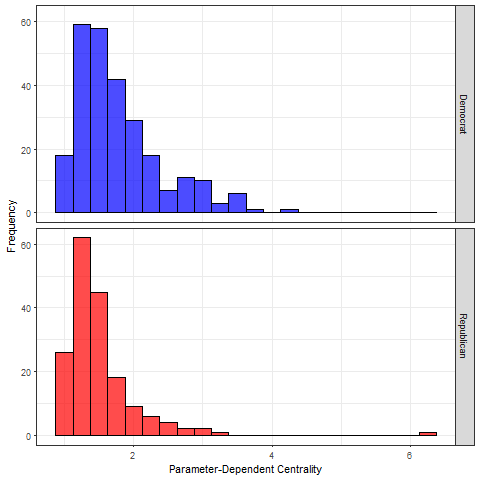
\includegraphics{Figure1}
		\caption{\label{fig:figure1} BLP model: Distribution of Parameter-Dependent Network Centrality.}
	\end{figure}
	Figure \ref{fig:figure1} can be replicated using the following script:
	\begin{CodeChunk}
		\begin{CodeInput}
			R> library("ggplot2")
			R> df <- data.frame(centrality = lim_centrality_model_B,
			+    party = lim_estimate_model_B$data$party1)
			R> df[, "party"] <- ifelse(df[, "party"] == 0, "Republican", 
			+    "Democrat")
			R> df[, "colour"] <- ifelse(df[, "party"] == "Republican", "red", 
			+    "blue")
			R> ggplot(data = df, aes(centrality), colour = df[, "colour"]) + 
			+    geom_histogram(binwidth = 0.25, aes(fill = factor(colour)), col = I("black"),
			+    alpha = I(.7)) + facet_grid(party ~.) + theme_bw() + 
			+    labs(x = "Parameter-Dependent Centrality", y = "Frequency") +
			+    scale_fill_manual(values = c("blue", "red")) + 
			+    theme(legend.position = "none")
		\end{CodeInput}
	\end{CodeChunk}
	\subsubsection{Exercise 2: Katz-Bonacich centrality with heterogenous by node parameter}
	
	The code below estimates model~\ref{BP_2} using gender as the
	relevant dimension of heterogeneity. Gender is a dummy variable
	which takes 1 if the legislator is a female, and 0 otherwise. 
	\begin{CodeChunk}
		\begin{CodeInput}
			R> z <- as.numeric(as.character(db_model_A[, "gender"]))
			R> f_het_model_A <- formula("PAC ~ party + nchair + isolate")
			R> starting <- c(alpha = 0.44835, beta_party1 = 0.56004,
			+    beta_nchair1 = -0.16349, beta_isolate1 = 0.21011,
			+    beta_z = -0.26015, phi = 0.34212, gamma = -0.49960)
			R> het_model_A <- net_dep(formula = f_het_model_A, data = db_model_A,
			+    G = G_model_A, model = "model_A", estimation = "NLLS",
			+    hypothesis = "het", z = z, start.val = starting)
			R > summary(het_model_A)
		\end{CodeInput}
		\begin{CodeOutput}
			Call:
			Main Equation:  
			Formula: PAC ~ alpha * solve_block(I - G %*% (phi * I + 
			gamma * G_heterogeneity)) %*% Ones + beta_party1 * party1 + 
			beta_nchair1 * nchair1 + beta_isolate1 * isolate1 + beta_z * z
			
			Parameters:
			Estimate Std. Error t value Pr(>|t|)    
			alpha          0.44835    0.17942   2.499   0.0128 *  
			beta_party1    0.56004    0.08342   6.713 6.21e-11 ***
			beta_nchair1  -0.16349    0.18984  -0.861   0.3896    
			beta_isolate1  0.21011    0.17927   1.172   0.2418    
			beta_z        -0.26014    0.10655  -2.441   0.0150 *  
			phi            0.34212    0.25377   1.348   0.1783    
			gamma         -0.49960    0.34662  -1.441   0.1502    
			---
			Signif. codes:  0 '***' 0.001 '**' 0.01 '*' 0.05 '.' 0.1 ' ' 1
			
			AIC: 1042.34  loglik: -513.17
		\end{CodeOutput}
	\end{CodeChunk}
	The results show that in this simple example $\gamma$\ is not significant, suggesting that female congressmen do not have a different level influence than their male peers. Note that the weighted Katz-Bonacich centrality derived from the spillover effect are stored in the object \code{het\_centrality\_model\_A.}
	
	If we use equation~\ref{BLP_3a} and~\ref{BLP_3b}, we distinguish between outgoing and incoming influence, that is if females are more (or less) able to influence and to be influenced by their peers respectively. The code below implements this analysis. For ease of exposition, we do not consider the possible endogeneity of the social network.
	\begin{CodeChunk}
		\begin{CodeInput}
			R> # Create gender variable
			R> z <- as.numeric(as.character(db_model_B[, "gender"]))
			R> # Specify formula
			R> f_het_model_B <- formula("les ~ party + nchair")
			R> # Specify starting values
			R> starting <- c(alpha = 0.23952, beta_party1 = 0.42947,
			+    beta_nchair1 = 3.09615, beta_z = -0.12749,
			+    theta_0 = 0.42588, theta_1 = 0.08007)
			R> # Run net_dep
			R> het_model_B_l <- net_dep(formula = f_het_model_B, data = db_model_B,
			+    G = G_model_B, model = "model_B", estimation = "NLLS",
			+    hypothesis = "het_l", z = z, start.val = starting)
			R> # Specify starting values
			R> starting <- c(alpha = 0.04717, beta_party1 = 0.51713,
			+    beta_nchair1 = 3.12683, beta_z = 0.01975,
			+    eta_0 = 1.02789, eta_1 = 2.71825)
			R> # Run net_dep
			R> het_model_B_r <- net_dep(formula = f_het_model_B, data = db_model_B,
			+    G = G_model_B, model = "model_B", estimation = "NLLS",
			+    hypothesis = "het_r", z = z, start.val = starting)
			R> # Store results in different objects
			R> het_l_estimate_model_B <- het_model_B_l[[1]]
			R> het_l_centrality_model_B <- het_model_B_l[[2]]
			R> het_r_estimate_model_B <- het_model_B_r[[1]]
			R> het_r_centrality_model_B <- het_model_B_r[[2]]
			R> # Print results
			R> summary(het_l_estimate_model_B)
		\end{CodeInput}
		\begin{CodeOutput}
			Call:
			Main Equation:  
			Formula: les ~ solve_block(I - (theta_0 * I - 
			theta_1 * G_heterogeneity) %*% G) %*% (alpha * Ones + 
			beta_party1 * party1 + beta_nchair1 * nchair1 + beta_z * z)
			
			Parameters:
			Estimate Std. Error t value Pr(>|t|)    
			alpha         0.22740    0.07584   2.998  0.00287 ** 
			beta_party1   0.41382    0.10198   4.058 5.88e-05 ***
			beta_nchair1  3.07797    0.26148  11.771  < 2e-16 ***
			beta_z       -0.12749    0.21199  -0.601  0.54789    
			theta_0       0.42587    0.07418   5.741 1.77e-08 ***
			theta_1       0.08007    0.12320   0.650  0.51611    
			---
			Signif. codes:  0 '***' 0.001 '**' 0.01 '*' 0.05 '.' 0.1 ' ' 1
			
			Residual standard error: 1.108 on 433 degrees of freedom
			
			AIC: 1343.68  loglik: -664.84
		\end{CodeOutput}
		\begin{CodeInput}
			R> summary(het_r_estimate_model_B)
		\end{CodeInput}
		\begin{CodeOutput}
			Call:
			Main Equation:  
			Formula: les ~ solve_block(I - G %*% (eta_0 * I - 
			eta_1 * G_heterogeneity)) %*% (alpha * Ones + 
			beta_party1 * party1 + beta_nchair1 * nchair1 + beta_z * z)
			
			Parameters:
			Estimate Std. Error t value Pr(>|t|)    
			alpha         0.04717    0.06867   0.687  0.49251    
			beta_party1   0.51713    0.09259   5.585 4.13e-08 ***
			beta_nchair1  3.12683    0.25680  12.176  < 2e-16 ***
			beta_z        0.01976    0.15098   0.131  0.89595    
			eta_0         1.02790    0.22400   4.589 5.85e-06 ***
			eta_1         2.71825    0.91547   2.969  0.00315 ** 
			---
			Signif. codes:  0 '***' 0.001 '**' 0.01 '*' 0.05 '.' 0.1 ' ' 1
			
			AIC: 1336.63  loglik: -661.31
		\end{CodeOutput}
	\end{CodeChunk}
	The results shows that females do not seem to be able to influence their socially connected peers ($\theta$ is not significant), but they are helpful to their colleagues ($\eta_{1}>0$). In terms of network analysis, this implies that all else being equal, congressmen located close to female colleagues benefit from their position since they can leverage females to be more effective in their legislative activity. In this case, the weighted Katz-Bonacich centralities are stored in \code{het\_l\_centrality\_model\_B}
	and \code{het\_r\_centrality\_model\_B}.
	
	\subsubsection{Exercise 3: Katz-Bonacich centrality with heterogenous by link parameter}
	
	In this last exercise, we show how to explore the hypothesis that relations within and between parties might have a different impact on the congressmen's LES. The code below estimates model~\ref{BLP_4} where the within and between effects are shaped by party membership.
	
	\begin{CodeChunk}
		\begin{CodeInput}
			R> # Specify partition vector
			R> z <- as.numeric(as.character(db_model_B[, "party"]))
			R> # Specify partition vector
			R> starting <- c(alpha = 0.242486, beta_gender1 = -0.229895,
			+    beta_party1 = 0.42848, beta_nchair1 = 3.0959,
			+    phi_within = 0.396371, phi_between = 0.414135)
			R> # Run net_dep
			R> party_model_B <- net_dep(formula = f_model_B,
			+    data = db_model_B,
			+    G = G_model_B, model = "model_B", estimation = "NLLS",
			+    hypothesis = "par", z = z, start.val = starting)
			R> # Store results in different objects
			R> party_estimate_model_B <- party_model_B[[1]]
			R> party_centrality_model_B <- party_model_B[[2]]
			R> # Print results
			R> summary(party_estimate_model_B)
		\end{CodeInput}
		\begin{CodeOutput}
			Call:
			Main Equation:  
			Formula: les ~ solve_block(I - phi_within * G_within - 
			phi_between * G_between) %*% (alpha * Ones + beta_gender1 * gender1 +
			beta_party1 * party1 + beta_nchair1 * nchair1)
			
			Parameters:
			Estimate Std. Error t value Pr(>|t|)    
			alpha         0.24249    0.08988   2.698 0.007251 ** 
			beta_gender1 -0.22990    0.14120  -1.628 0.104221    
			beta_party1   0.42848    0.12623   3.394 0.000751 ***
			beta_nchair1  3.09590    0.26008  11.904  < 2e-16 ***
			phi_within    0.39637    0.07306   5.425 9.66e-08 ***
			phi_between   0.41414    0.24175   1.713 0.087420 .  
			---
			Signif. codes:  0 '***' 0.001 '**' 0.01 '*' 0.05 '.' 0.1 ' ' 1
			
			AIC: 1344.1  loglik: -665.05
		\end{CodeOutput}
	\end{CodeChunk}
	
	
	The estimation results show that connections within one's own party and between parties are both significant for advancing a piece of legislation. The weighted Katz-Bonacich centrality can be found in the object \code{party\_centrality\_model\_B}.
	
	\subsection{Centrality measure comparison}
	
	The \proglang{R} package \pkg{econet} allows also to evaluate the explanatory power of parameter-dependent centralities relative to other centrality measures, which depends on network topology only. More specifically, \pkg{econet} considers the following measures, which are computed using the \proglang{R} package \code{igraph} \citep{igraph}: indegree centrality, outdegree centrality, degree centrality, betweenness centrality, incloseness centrality, outcloseness centrality, closeness centrality. It also reports eigenvector centrality, which is calculated using the \proglang{R} package \pkg{sna} \citep{sna}.\footnote{Indegree centrality is the number of incoming links of one node; outdegree centrality is the number of outgoing links of one node; degree centrality is the sum of in and out degree; betweenness centrality is the number of times a node falls on the shortest path between two other nodes; incloseness centrality is the inverse of the average distance of one node from all the other nodes passing through incoming links; outcloseness centrality is the inverse of the average distance of one node from all the other nodes passing through outcoming links; closeness centrality is the sum of in and out closeness, and eigenvector centrality is proportional to the sum of the centrality of agent's neighbors \cite[see][for further details]{Jackson:2010}.}
	We then implement an augmented version of models~\ref{NLLS} and~\ref{BLP} where we add one (or more) centrality measures in the matrix of individual characteristics $X_{r}^\top.$ By doing so we can run an horse race across different centrality measures.
	
	The arguments of the function \code{horse\_race} are similar to the \code{net\_dep} ones. The different ones are: i) \code{centralities}, an object or a vector of class \code{character} specifying the names of the centrality measure(s) to be used; ii) \code{directed}, a logical object
	which is set to \code{TRUE} if the network is directed, and \code{FALSE} otherwise; iii) \code{weighted}, a logical object equal to \code{TRUE} if links between agents have weights, and \code{FALSE} otherwise; and iv) \code{normalization}, an object
	of class character which can be used to normalize centrality measures before the estimations. \footnote{The options available are: \code{NULL}, no normalization; \code{bygraph}, divide by the number of nodes in the network minus 1 (for degree and closeness) or the number of possible links in the network (betweenness), \code{bycomponent}, divide by the number of nodes in agent's component minus 1 (for degree and closeness) or the number of possible links in agent's component (betweenness); \code{bymaxgraph}, divide by the maximum centrality value in the network; \code{bymaxcomponent}, divide by the maximum centrality value in agent's component.}
	
	The output of this function is also similar to \code{net\_dep}, i.e., a list containing the results of the main estimates in the first object, a \code{data.frame} listing the centrality measures in the second object, and the results of the first step estimation in the third object (if \code{endogeneity = TRUE}). An example of how this model is implemented and results are stored is provided in the following example, where we use a linear regression model where betweenness centrality is a regressor.
	
	\begin{CodeChunk}
		\begin{CodeInput}
			R> starting <- c(alpha = 0.214094, beta_gender1 = -0.212706,
			+    beta_party1 = 0.478518, beta_nchair1 = 3.09234,
			+    beta_betweenness = 7.06287e-05, phi = 0.344787)
			R> example_model <- lm(response ~ variable1 + variable2 + variable3, 
			R> horse_model_B <- horse_race(formula = f_model_B, 
			+    centralities = "betweenness", directed = TRUE, weighted = TRUE, 
			+    normalization = NULL, data = db_model_B, G = G_model_B,
			+    model = "model_B", estimation = "NLLS", start.val = starting)
			R> summary(horse_model_B, centrality = "betweenness")
		\end{CodeInput}
		\begin{CodeOutput}
			Call:
			Main Equation:  les ~ gender + party + nchair + betweenness
			
			Residuals:
			Min      1Q  Median      3Q     Max 
			-3.6051 -0.5665 -0.1877  0.2559 10.8641 
			
			Coefficients:
			Estimate Std. Error t value Pr(>|t|)    
			(Intercept)  3.300e-01  9.042e-02   3.650 0.000295 ***
			gender1     -8.904e-02  1.445e-01  -0.616 0.538011    
			party1       7.054e-01  1.139e-01   6.194 1.36e-09 ***
			nchair1      3.202e+00  2.644e-01  12.112  < 2e-16 ***
			betweenness  1.851e-04  3.985e-05   4.645 4.51e-06 ***
			---
			Signif. codes:  0 '***' 0.001 '**' 0.01 '*' 0.05 '.' 0.1 ' ' 1
			
			AIC: 1362.19  loglik: -675.09
		\end{CodeOutput}
		\begin{CodeInput}
			> summary(horse_model_B)
		\end{CodeInput}
		\begin{CodeOutput}
			Call:
			Main Equation:
			Formula: les ~ solve_block(I - phi * G) %*% (alpha * Ones + 
			beta_gender1 * gender1 + beta_party1 * party1 + 
			beta_nchair1 * nchair1 + beta_betweenness * betweenness)
			
			Parameters:
			Estimate Std. Error t value Pr(>|t|)    
			alpha             2.141e-01  7.676e-02   2.789  0.00552 ** 
			beta_gender1     -2.127e-01  1.408e-01  -1.511  0.13162    
			beta_party1       4.785e-01  1.105e-01   4.331 1.85e-05 ***
			beta_nchair1      3.092e+00  2.593e-01  11.927  < 2e-16 ***
			beta_betweenness  7.063e-05  4.561e-05   1.549  0.12219    
			phi               3.448e-01  7.101e-02   4.856 1.68e-06 ***
			---
			Signif. codes:  0 '***' 0.001 '**' 0.01 '*' 0.05 '.' 0.1 ' ' 1
			
			AIC: 1341.61  loglik: -663.8
		\end{CodeOutput}
	\end{CodeChunk}
	
	The results of this estimation show evidence that being able to broker connections in the network, as measured by betweenness centrality in the object \code{summary(horse_model_B)}
	is associated with higher legislative effectiveness. The effect disappears when we include network effects, that is when we add betweenness centrality as an additional regressor in the linear model of social interactions (equation~\ref{BLP}). This suggests that Katz-Bonacich centrality is a more robust predictor of effectiveness in this context. Estimates are stored in the object \code{horse\_estimate\_model\_B}, whereas centrality measures in the object \code{horse_model_B\$centrality}.
	
	\section{Conclusions}
	
	We have described the key elements for the estimation of parameter-dependent centralities derived from equilibrium models of behavior, and discussed the use of the package \pkg{econet} for the implementation of such metrics. The methods described in the paper are derived from several modifications to the linear-in-means model - for which both nonlinear least squares
	and maximum likelihood estimators are provided - and they allow one to model both link and node heterogeneity in network effects, endogenous network formation and the presence of unconnected nodes. Furthermore, they provide the means to compare the explanatory power of parameter-dependent network centrality measures with those of standard measures of network
	centrality. A number of examples are used to walk the reader through the discussion and orientate the application of these methods to new potential directions of research.
	
\bibliography{econet_refs}

\end{document}
